

		
\includegraphics[scale=0.1]{Images/jenkins.jpeg} 
		Jenkins.

		This plugin was quite easy to choose, it fills exactly the need of the 
		company. 
		This application provides an easy to use continuous integration system. 
		It is an application that monitors executions of repeated jobs such as bulding, testing a software project.
		It has 3 main features : 
		\begin{itemize}
			\item It allows a team to share common information easily.
			\item It executes automatically compilation, testing without human intervention.
			\item It keeps a track of previous productions and allow us to see their development. 
		\end{itemize}


		
\includegraphics[scale=0.2]{Images/mylin.jpeg} 
		Mylin for eclipse connection. 

		Here too, the plugin fits exactly the need of the company. It is the only
		one that allow users to have a connection to Redmine from Eclipse.
		Mylin is the task and application lifecycle management framework for Eclipse.
		It allows to visualize tasks from Redmine repository and it has a 
		connector to Jenkins. \\ 
		It helps a developer to work efficiently with many different tasks 
		(such as bugs, problem reports or new features). In a nutshell, 
		it improves their productivity by reducing searching, scrolling, and 
		navigation. \\

		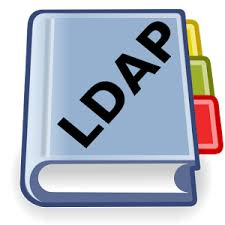
\includegraphics[scale=0.1]{Images/ldap.jpeg} 
		Ldap authentification. 

		Ldap is a protocol that allow us to access and maintain directory services. So we can access to some informations about the users of a network over TCP/IP protocol. 
		With the ldap authentification into redmine, the users don't need to create a Redmine's account but they can directly access into their redmine's project by using their ldap password and login.   
		It just makes the register part into Redmine easier and faster.
